\documentclass[border=4pt,varwidth=17cm]{standalone}
\usepackage{amsmath,amssymb,mathrsfs,mathtools}
\usepackage{tikz}
\usetikzlibrary{positioning,fit,backgrounds,arrows.meta}
\def\RR{{\mathbb R}}\def\eps{\varepsilon}\def\then{\Rightarrow}
\def\J{\mathcal{J}_L}\def\A{\mathcal{A}_{f,g}}\def\Sol{\mathcal{S}_{f,g}}
\def\limsup{\mathop{\overline{\lim}}}\def\liminf{\mathop{\underline{\lim}}}
\def\Of{{\sf (O$_f$)}}\def\Og{{\sf (O$_g$)}}
\def\Rv{{\sf (R$_{\rm v}$)}}\def\Rh{{\sf (R$_{\rm h}$)}}
\begin{document}


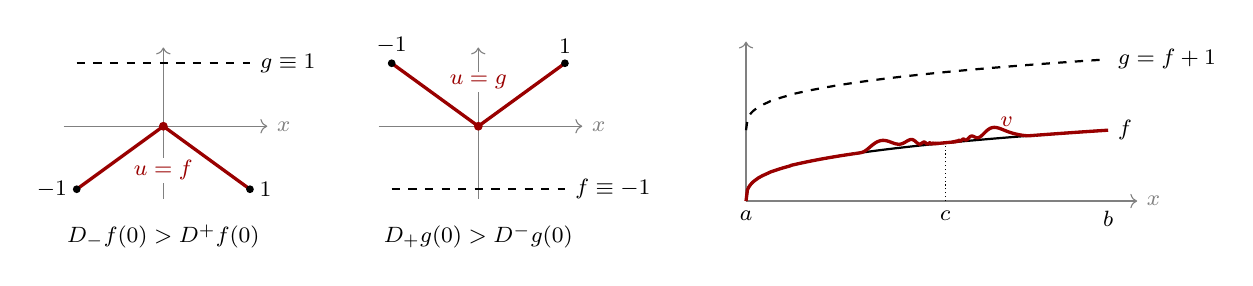
\begin{tikzpicture}[font=\footnotesize]
% (b) concave corner of f
\begin{scope}[x=1.1cm, y=0.8cm]
  \draw[->, gray] (-1.15,0) -- (1.2,0) node[right] {$x$};
  \draw[->, gray] (0,-1.15) -- (0,1.25);
  \draw[thick, dashed] (-1,1) -- (1,1) node[right] {$g\equiv1$};
  \draw[very thick, red!60!black] (-1,-1) -- (0,0) -- (1,-1);
  \node[red!60!black, fill=white, inner sep=1pt] at (0,-0.7) {$u=f$};
  \fill (-1,-1) circle (1.4pt) node[left] {$-1$};
  \fill (1,-1) circle (1.4pt) node[right] {$1$};
  \fill[red!60!black] (0,0) circle (1.6pt);
  \node[align=center] at (0,-1.75) {$D_-f(0)>D^+f(0)$};
\end{scope}
% (b) convex corner of g
\begin{scope}[shift={(4.0,0)}, x=1.1cm, y=0.8cm]
  \draw[->, gray] (-1.15,0) -- (1.2,0) node[right] {$x$};
  \draw[->, gray] (0,-1.15) -- (0,1.25);
  \draw[thick, dashed] (-1,-1) -- (1,-1) node[right] {$f\equiv-1$};
  \draw[very thick, red!60!black] (-1,1) -- (0,0) -- (1,1);
  \node[red!60!black, fill=white, inner sep=1pt] at (0,0.7) {$u=g$};
  \fill (-1,1) circle (1.4pt) node[above] {$-1$};
  \fill (1,1) circle (1.4pt) node[above] {$1$};
  \fill[red!60!black] (0,0) circle (1.6pt);
  \node[align=center] at (0,-1.75) {$D_+g(0)>D^-g(0)$};
\end{scope}
% (c) infinite energy
\begin{scope}[shift={(7.4,-0.95)}, x=4.6cm, y=0.9cm,
  declare function={F(\t)=\t^(1/3); W(\t)=4.5*exp(1-1/(1-((\t-0.55)/0.25)^2))*(\t-0.55)^2*(2+sin(deg(1/(\t-0.55))));}]
  \draw[->, gray] (0,0) -- (1.08,0) node[right] {$x$};
  \draw[->, gray] (0,0) -- (0,2.25);
  \draw[thick, domain=0:1, samples=200, smooth] plot (\x, {F(\x)}) node[right] {$f$};
  \draw[thick, dashed, domain=0:1, samples=200, smooth] plot (\x, {F(\x)+1}) node[right] {$g=f+1$};
  \draw[very thick, red!60!black, domain=0:0.301, samples=80] plot (\x, {F(\x)});
  \draw[very thick, red!60!black, domain=0.301:0.53, samples=300] plot (\x, {F(\x)+W(\x)});
  \draw[very thick, red!60!black] (0.53,{F(0.53)+W(0.53)}) -- (0.57,{F(0.57)+W(0.57)});
  \draw[very thick, red!60!black, domain=0.57:0.799, samples=300] plot (\x, {F(\x)+W(\x)});
  \draw[very thick, red!60!black, domain=0.799:1, samples=60] plot (\x, {F(\x)});
  \node[red!60!black] at (0.72,1.12) {$v$};
  \draw[densely dotted] (0.55,0) node[below] {$c$} -- (0.55,{F(0.55)});
  \node[below] at (0,0) {$a$};
  \node[below] at (1,0) {$b$};
\end{scope}
\end{tikzpicture}


\end{document}
